\documentclass{article}
%Paquete para agregar imagenes
\usepackage{graphicx}
%Paquete para usar la opcion H (posicion) en las imagenes
\usepackage{float}
%Ruta de las capturadas utilizadas
\graphicspath{ {capturas/tunelssh} }

\title{Practica 3: Ataque ARP Spoofing y tunneling con SSH}
\author{Juan Carlos Perales de Jes\'us, Yafte Aaron Flores, Ra\'ul C\'astulo Ortega}
\date{19 Octubre 2017}
\
\makeindex

\begin{document}
\maketitle
\newpage

\section{Res\'umen}

\section{Introducci\'on}
Cuando un equipo pertenece a una red es posible que \'este pueda ver el tr\'afico de la red, si la navegaci\'on no es segura, dicho equipo puede ver en claro la informaci\'on que se envía por la red.
 
\section{Objetivo}
Cifrar un canal de comunicaci\'on para navegar por la red aun por sitios no seguros.

\section{Planteamiento del problema}
Con herramientas de sniffering como Wireshark es posible ver el tr\'afico de la red, para evitar mandar paquetes con informaci\'on en claro, blindaremos el canal de comunicaci\'on.

\section{Metodolog\'ia a emplear}
Crearemos un tunel SSH para redirigir el trafico de la red a traves de otra maquina, el flujo de paquetes pasar\'a por un canal SSH, el cual es cifrado, \'esto evitara enviar paquetes en claro por la red.

\section{Materiales}
\begin{enumerate}
\item M\'aquina virtual con Kali-Linux
\item Sistema Operativo Windows \(7,8,10\)
\item Putty
\item OpenSSH
\item Wireshark
\item Navegador Web Firefox
\end{enumerate}

\section{Desarrollo}Los siguientes pasos se llevarón a cabo desde el sistema operativo Windows 10, con una maquina virtual con Kali linux.

\subsection{Obtener IP de m\'aquina host (windows) y maquina virtual (kali linux)}
En Windows abrimos la l\'inea de comandos de windows \emph{cmd} y tecleamos \emph{ipconfig}
En este caso la IP del host es \emph{192.168.0.102}

%Imagen 1
\begin{figure}[H]
\centering
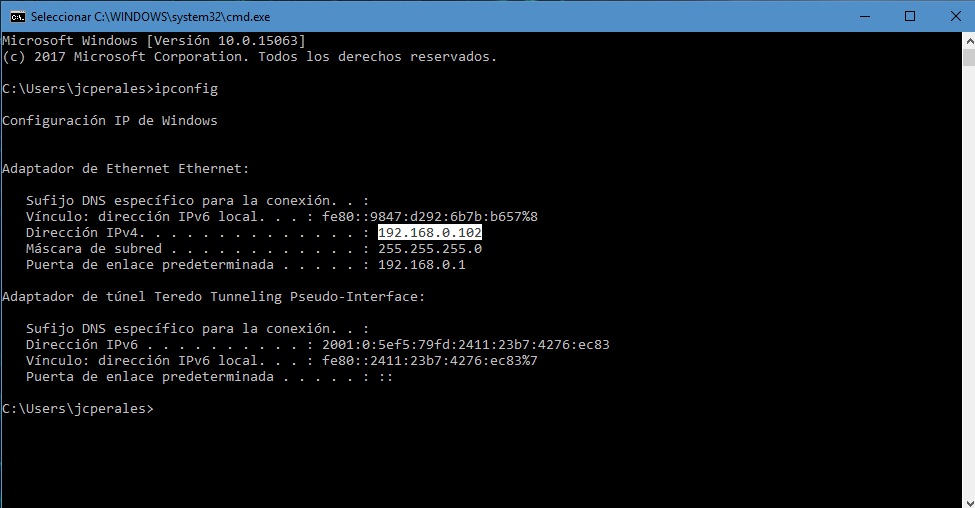
\includegraphics[width=1\textwidth]{01-IPCONFIG}
\end{figure}

En la maquina virtual abrimos una terminal y ejecutamos el comando \emph{ifconfig}, la interfaz eth0 nos reporta la direcci\'on IP \emph{10.0.2.15}

%Imagen 2
\begin{figure}[H]
\centering
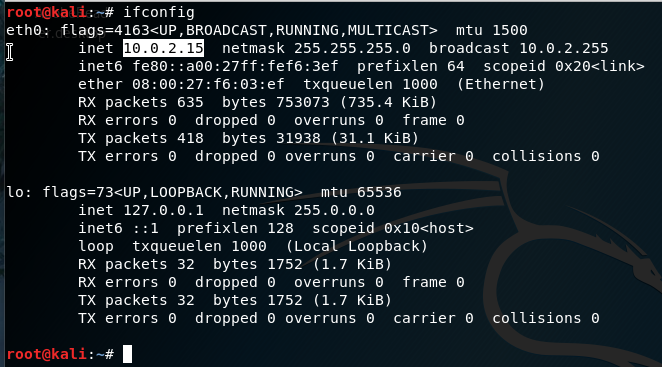
\includegraphics[width=1\textwidth]{02-IFCONFIG}
\end{figure}


\subsection{Configuraci\'on de VirtualBox}

Ya que conocemos ambas direcciones IP, en Virtualbox nos vamos a \emph{Dispositivos/Red/Preferencias de Red}

%Imagen 3
\begin{figure}[H]
\centering
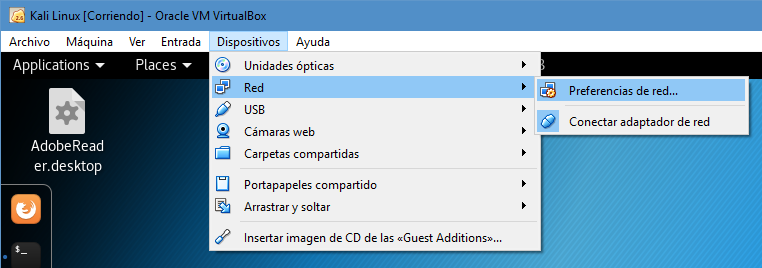
\includegraphics[width=1\textwidth]{03-PREFERENCIADERED}
\end{figure}

Desp\'ues damos clic en el bot\'on que dice \emph{Reenvio de Puertos}

%Imagen 4
\begin{figure}[H]
\centering
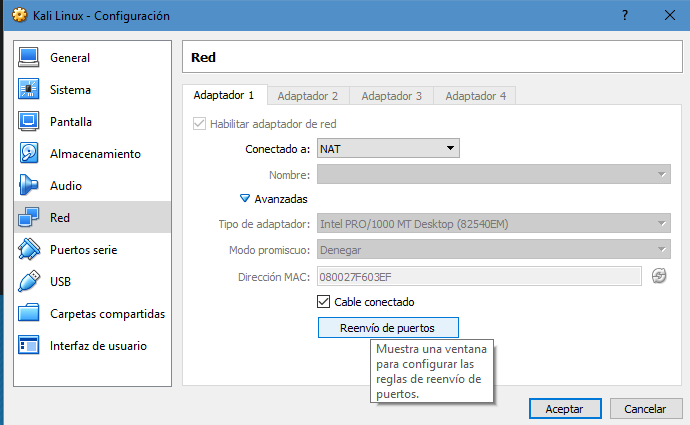
\includegraphics[width=1\textwidth]{04-REENVIOPUERTOS}
\end{figure}

Por \'ultimo agregamos una regla con los datos como se muestra a continuaci\'on: 

%Imagen 5
\begin{figure}[H]
\centering
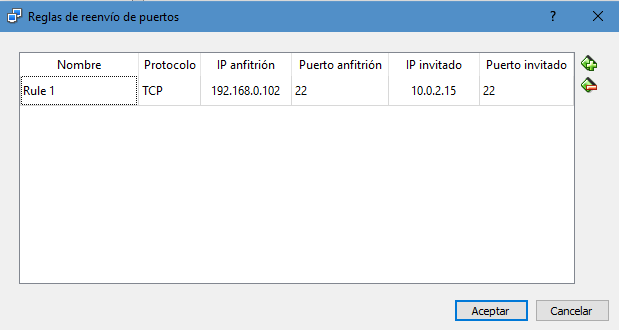
\includegraphics[width=1\textwidth]{05-CONFIGURADO}
\end{figure}

\subsection{Configuraci\'on servidor SSH en Kali linux}

En la terminal de Kali editamos del archivo \emph{/etc/ssh/sshd\_config} la linea \emph{PermitRootLogin} y cambiamos su valor a \emph{yes}

%Imagen 6
\begin{figure}[H]
\centering
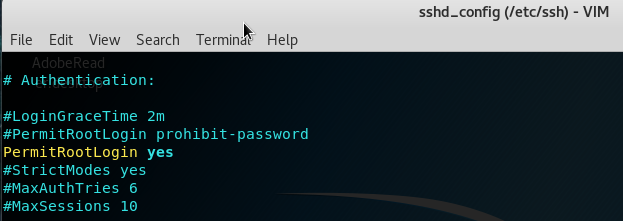
\includegraphics[width=1\textwidth]{06-CONFIGURACIONSSHD}
\end{figure}

Por \'ultimo inicializamos el demonio, para ello tecleamos en la terminal \emph{/etc/init.d/ssh start}

%Imagen 7
\begin{figure}[H]
\centering
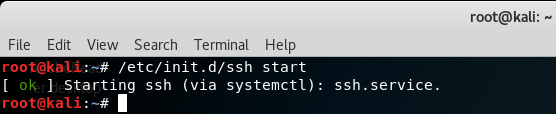
\includegraphics[width=1\textwidth]{07-STARTSSHD}
\end{figure}

Ya tenemos el servidor SSH listo para que accedamos desde Putty.

\subsection{Configuraci\'on de tunel SSH con Putty}

Abrimos Putty y tecleamos la IP a la que queremos conectarnos y dejamos el puerto estandar de ssh que es el 22 (ya configuramos virtualbox para que redirija las peticiones del puerto 22 a la maquina virtual). Una vez ingresado la IP y el puerto, guardamos la sesi\'on.

%Imagen 8
\begin{figure}[H]
\centering
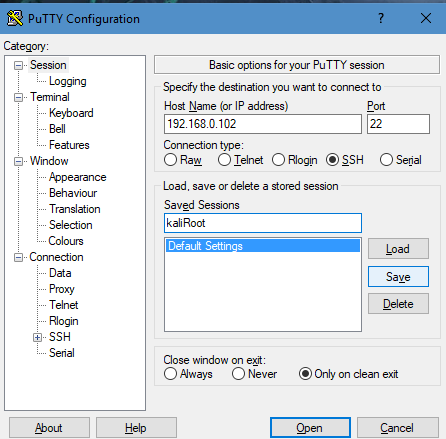
\includegraphics[width=1\textwidth]{08-GUARDARKALIPUTTY}
\end{figure}

Hacemos una prueba para ver que el servidor SSH de la maquina virtual funciona correctamente, nos conectamos y nos logeamos con nuestras credenciales.

%Imagen 9
\begin{figure}[H]
\centering
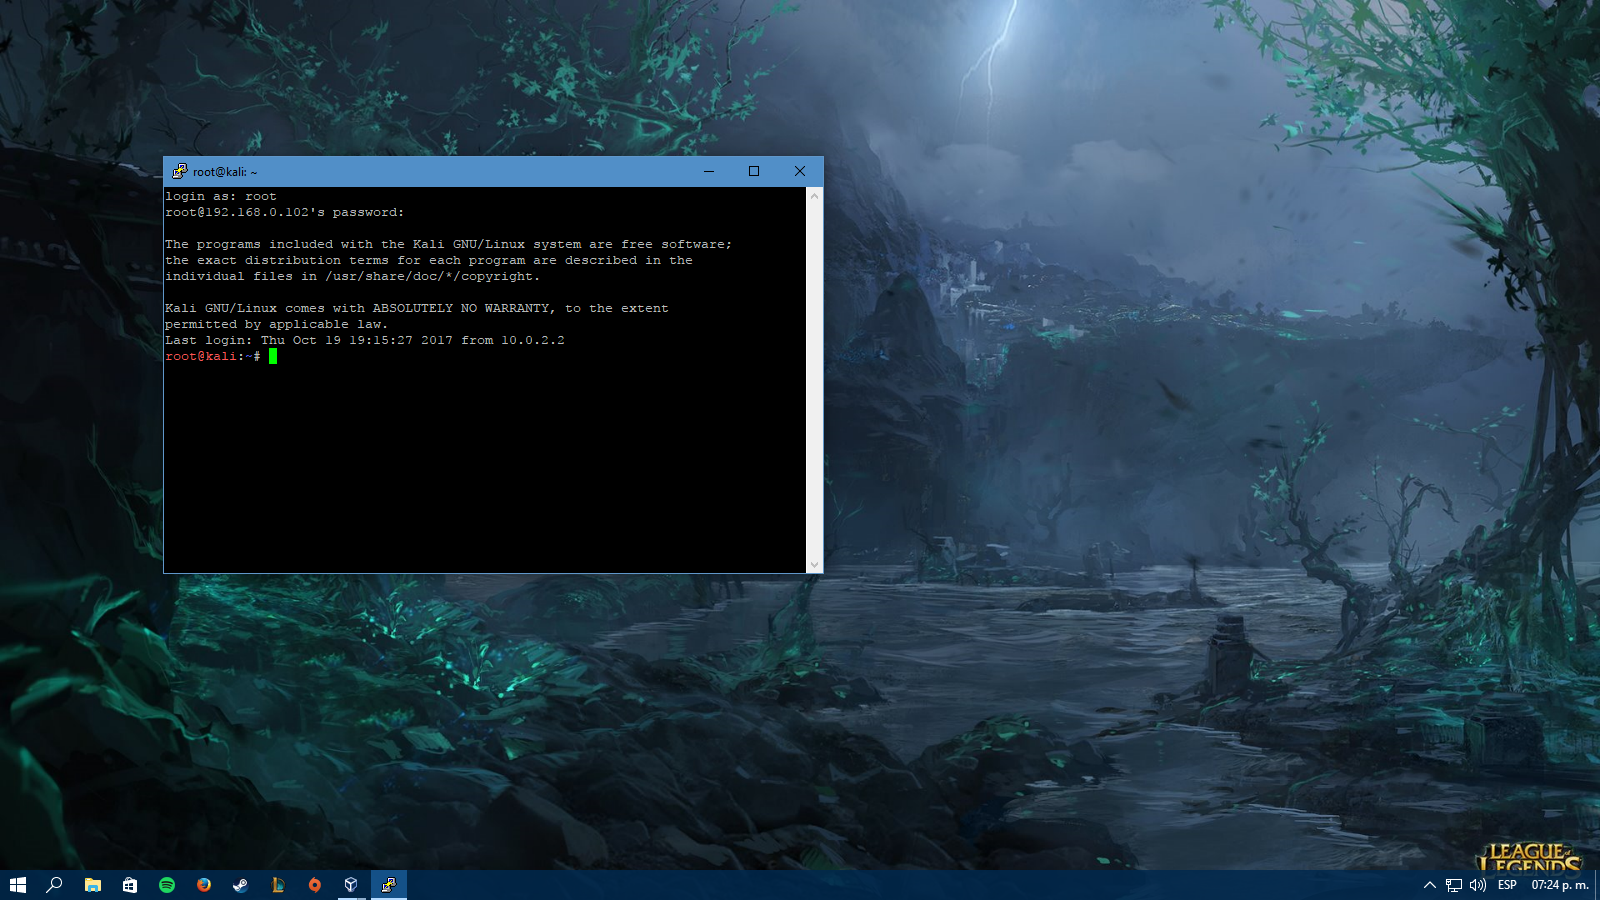
\includegraphics[width=1\textwidth]{09-LOGEADOSSH}
\end{figure}

Ya que pudimos acceder a la maquina virtual por medio de SSH, ahora cargamos la sesion que guardamos previamente y nos vamos al apartado \emph{Conection/SSH/Tunnels} en Putty. Ahí agregamos un puerto, en nuestro caso utilizamos el puerto \emph{50000}, marcamos la opcion \emph{Dynamic},le damos clic al boton \emph{Add} y por ultimo nos conectamos de igual manera al paso anterior.

%Imagen 10
\begin{figure}[H]
\centering
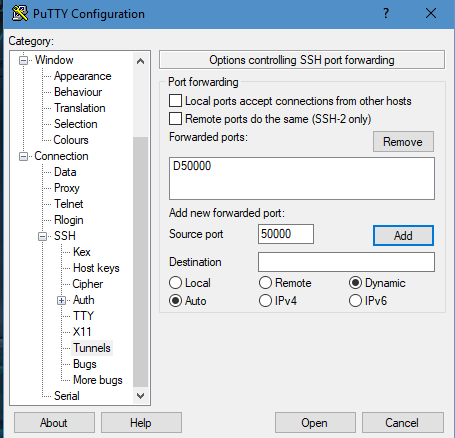
\includegraphics[width=1\textwidth]{10-PUERTO50000}
\end{figure}

\subsection{Configuraci\'on de Firefox}

Despu\'ues de preparar el tunel SSH, tenemos que configurar nuestro navegador para redirigir el trafico a traves del tunel. Para lo anterior nos vamos a las opciones de Firefox

%Imagen 11
\begin{figure}[H]
\centering
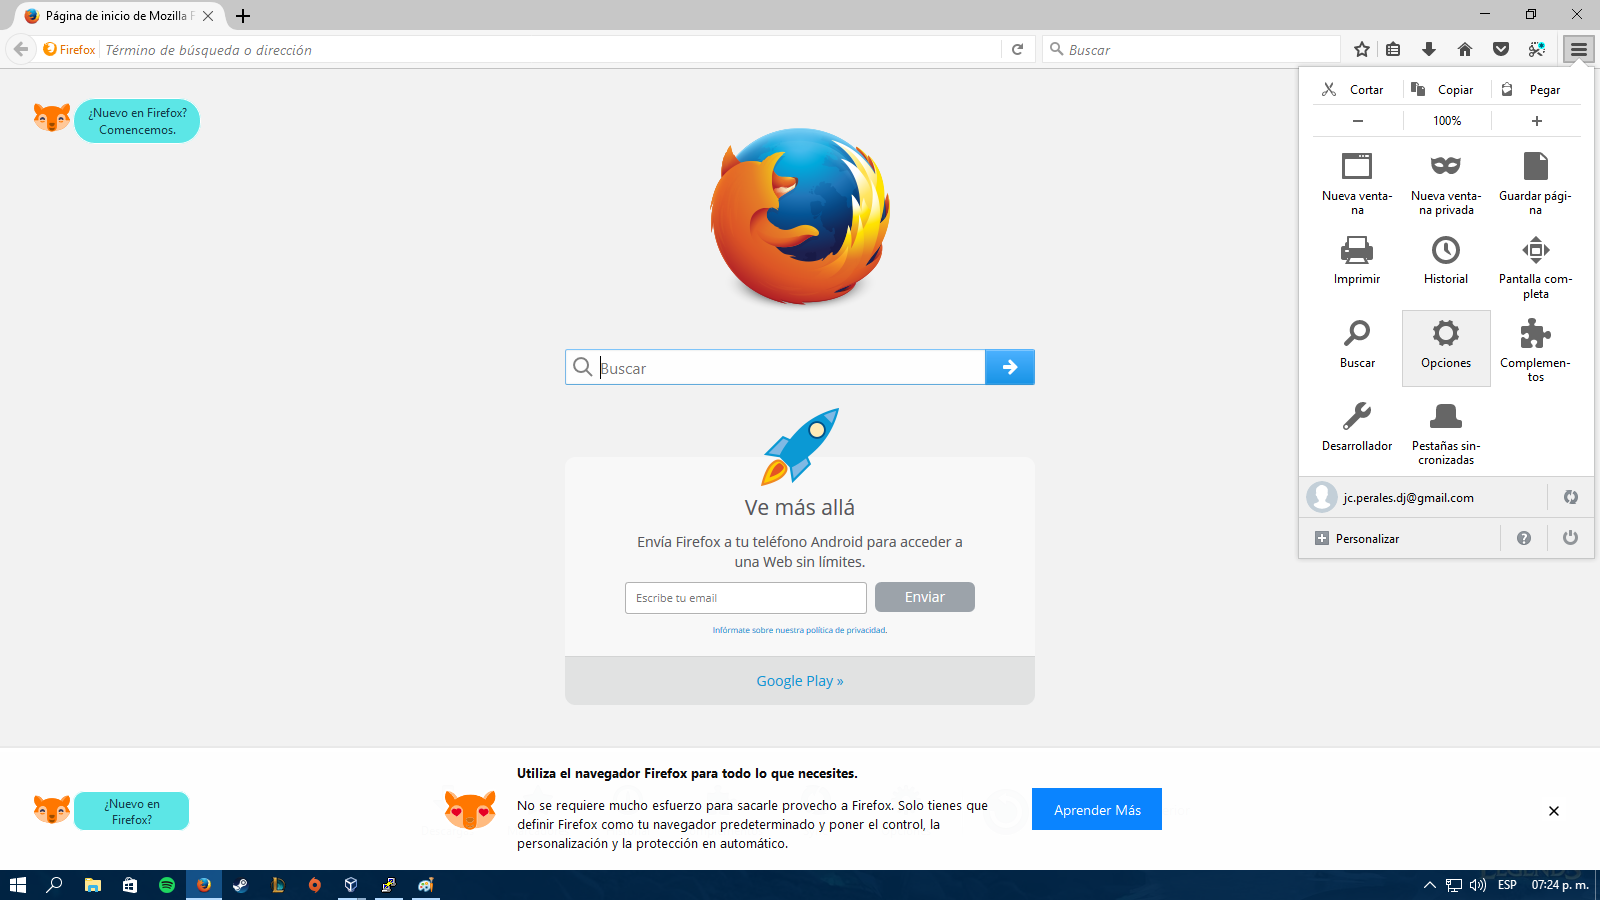
\includegraphics[width=1\textwidth]{11-OPCIONESFIREFOX}
\end{figure}

En la pestaña general, nos vamos a la secci\'on que dice \emph{Proxy de red} y damos clic en el boton \emph{Configurar...}

%Imagen 12
\begin{figure}[H]
\centering
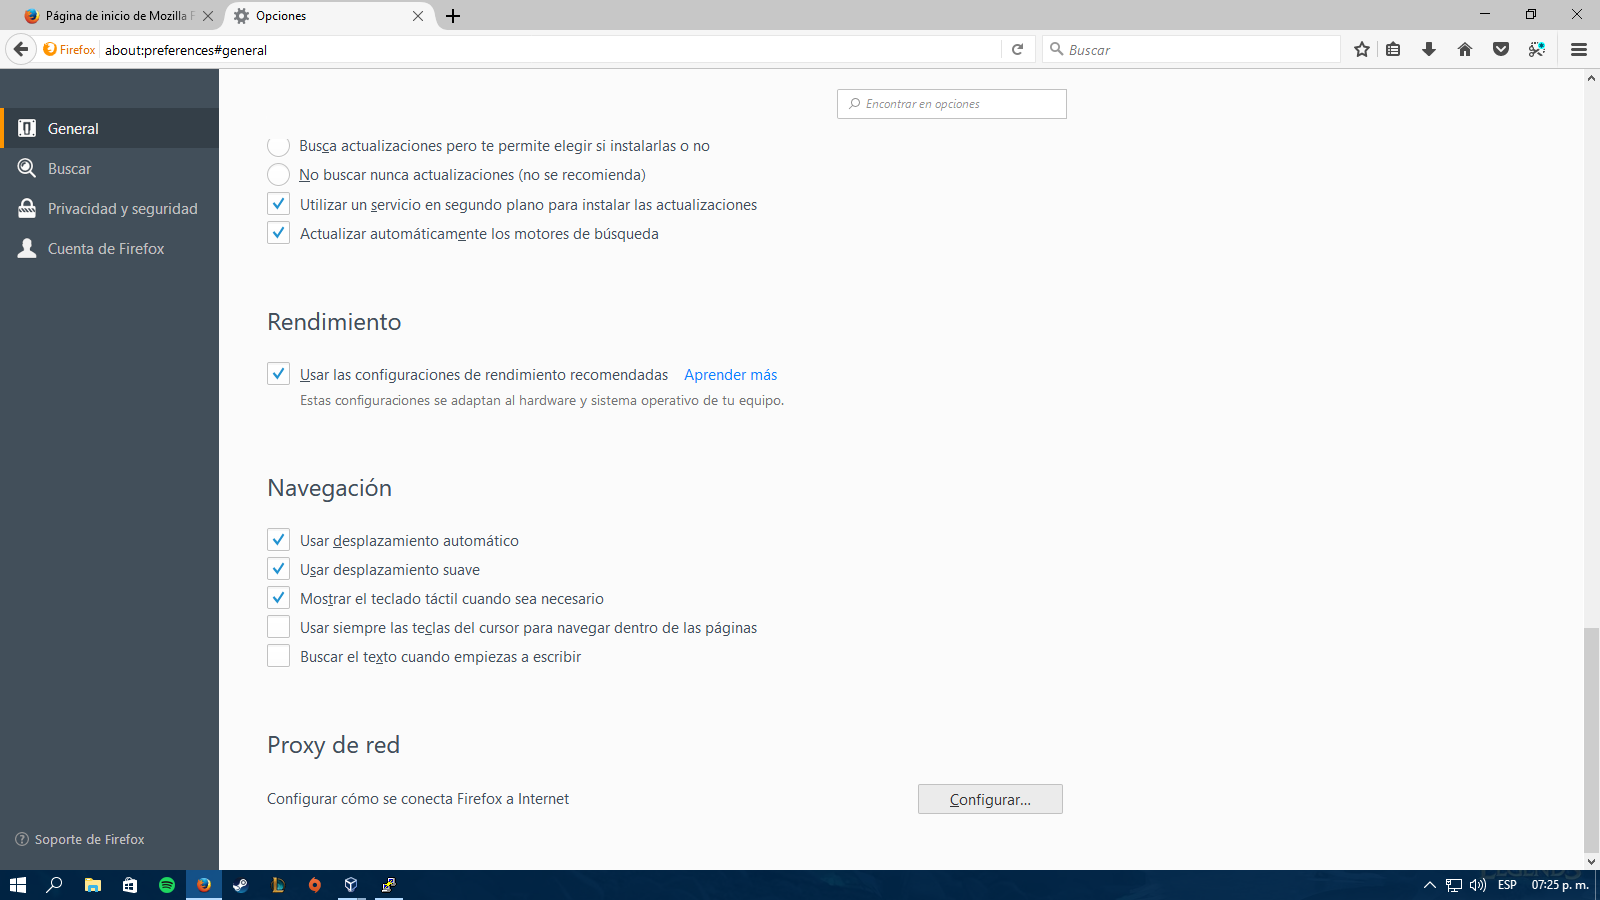
\includegraphics[width=1\textwidth]{12-CONFIGURACIONPROXY}
\end{figure}

Por ultimo marcamos la casilla que dice \emph{Configuracion manual del proxy:} y en el cuadro de texto que dice \emph{Servidor SOCKS} ingresamos la IP \emph{127.0.0.1} (direcci\'on loopback) y en puerto asignamos el mismo que configuramos en Putty, es decir el \emph{50000}. 

%Imagen 13
\begin{figure}[H]
\centering
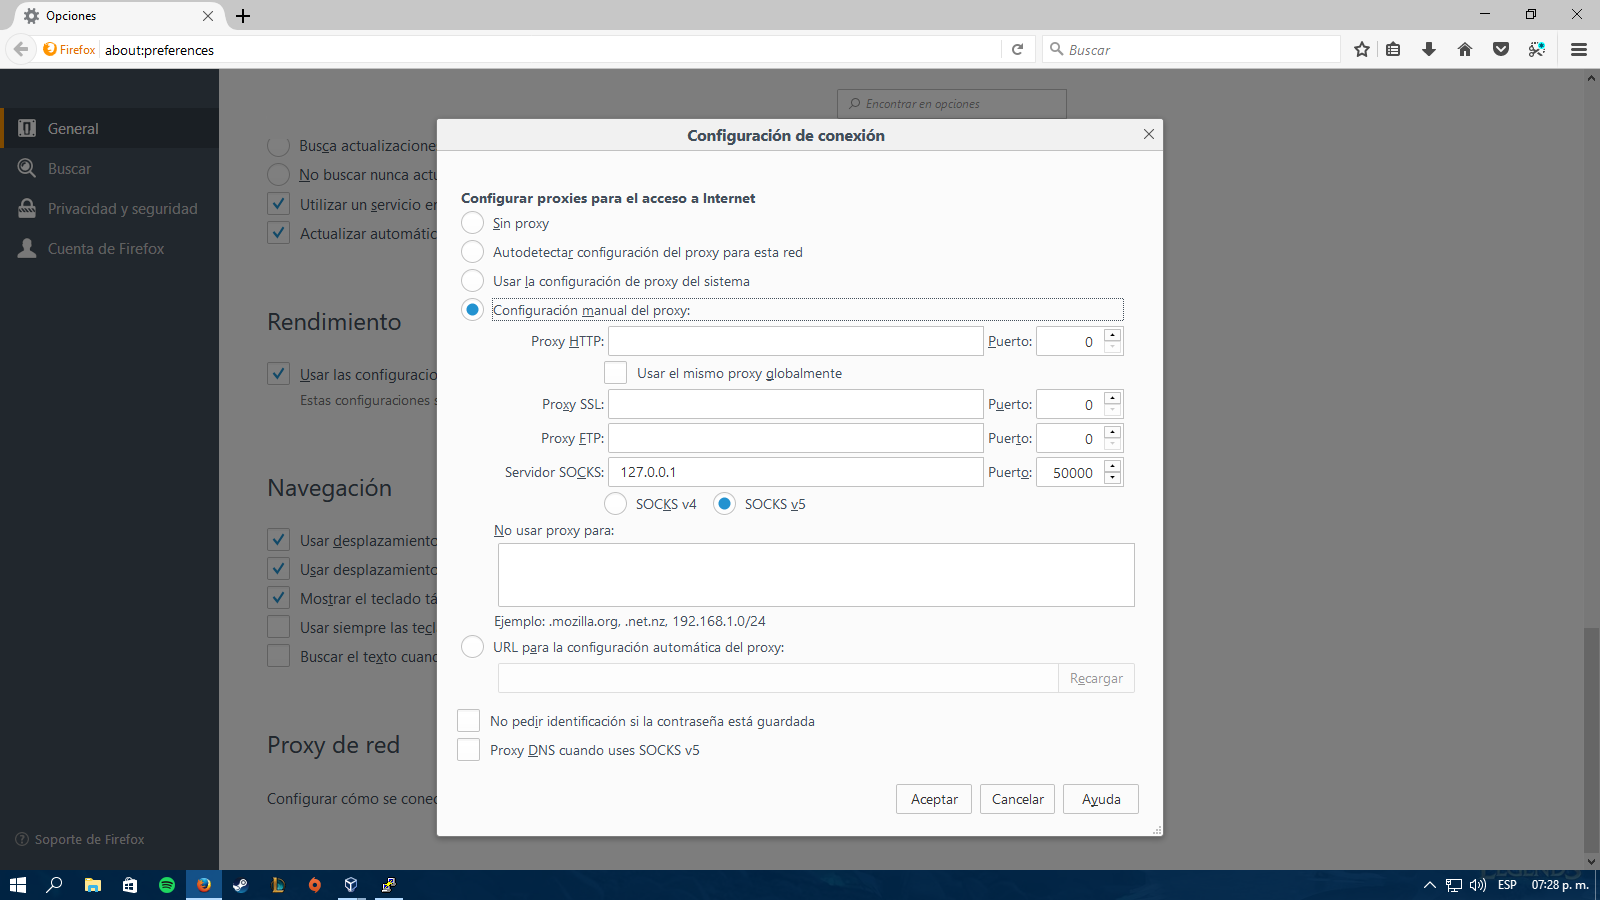
\includegraphics[width=1\textwidth]{13-CONFIGURACIONSOCKS}
\end{figure}

Damos clic en \emph{Aceptar} y listo, tenemos nuestro tunel SSH que pasa todo el trafico enviado por Firefox en la maquina host a la maquina virtual kali linux de manera encriptada.

\section{Resultados}

\section{Discusi\'on}

\section{Conclusiones}

\section{Bibliograf\'ia}

\end{document}